\documentclass{beamer}
\usepackage{graphicx}
\usepackage{listings}
\usepackage{hyperref}
\usepackage[autostyle, english=american]{csquotes}
\MakeOuterQuote{"}
\usetheme{Pittsburgh}

\setbeamertemplate{caption}[numbered]

% \definecolor{maincs}{RGB}{0,255,0}
% \definecolor{secondarycs}{RGB}{255,179,246}
\definecolor{purple}{rgb}{0.65, 0.12, 0.82}

\lstset{
    language=Python,
        basicstyle=\fontsize{9}{10}\ttfamily,
        otherkeywords={self,import,from},
        keywordstyle=\color{purple}\ttfamily,
        emph={True,False},
        emphstyle=\color{orange},
        stringstyle=\color{red}\ttfamily,
        commentstyle=\color{blue}\ttfamily,
        morecomment=[l][\color{blue}]{\#},
        tabsize=2,
        showstringspaces=false
}

\title{Raspberry Pi Watering System}
\author{Caleb Jhones}
\date{30 November 2017}
\institute{CSCI 250}

\begin{document}

\begin{frame}
    \maketitle
\end{frame}

\begin{frame}
    \frametitle{Purpose}
    \begin{minipage}{0.45\textwidth}
        \begin{figure}
            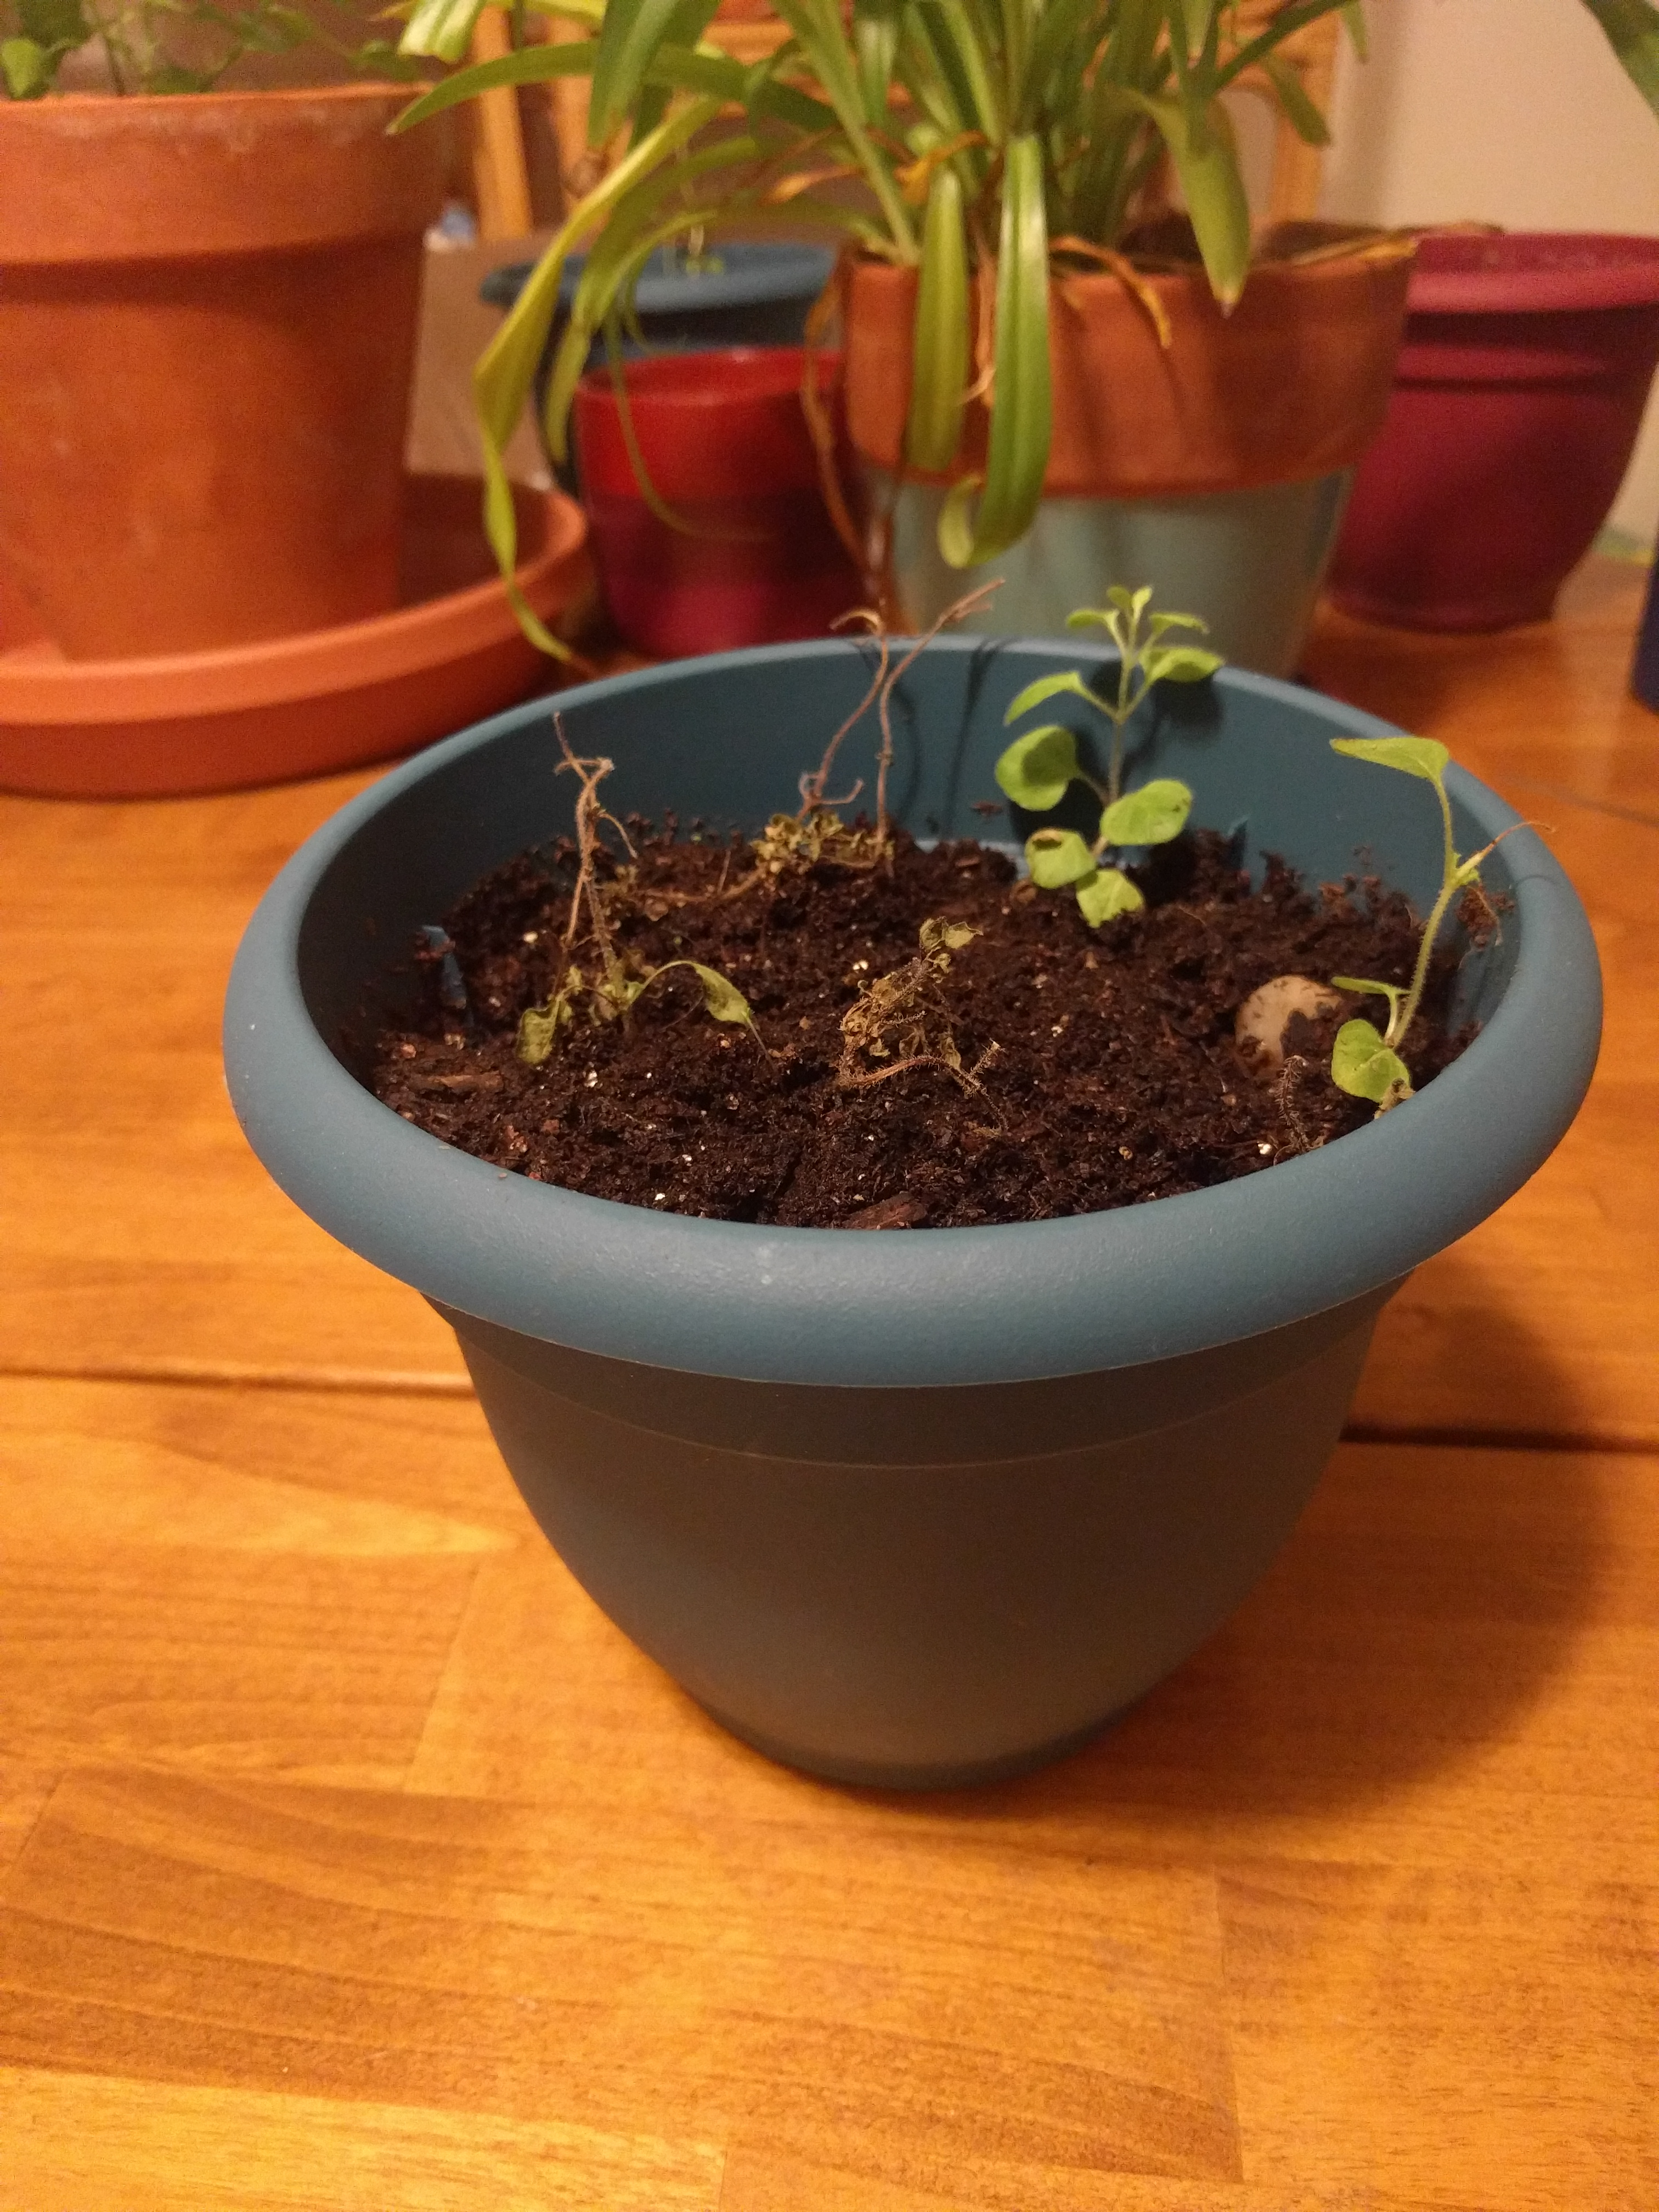
\includegraphics[width=5cm]{../img/sad-plants}
            \caption{Sad plants :(}
        \end{figure}
    \end{minipage}%
    \begin{minipage}{0.55\textwidth}
        \begin{itemize}
            \item Turns out, I have a brown thumb...
            \pause
            \item But I like growing things!
            \pause
            \item So why not use technology to help water my plants?
        \end{itemize}
    \end{minipage}%
\end{frame}

\begin{frame}
    \frametitle{Parts Used}
    \begin{itemize}
        \item 1x Raspberry Pi
        \item 1x \href{https://www.amazon.com/gp/product/B01FDGUHBM}{Soil Hygrometer Sensor}
        \item 1x \href{https://www.sparkfun.com/products/10456}{12V Solenoid}
        \item 1x \href{https://www.sparkfun.com/products/13815}{Sparkfun Relay}
        \item 1x 5V Power supply (for the Pi and the hygrometer)
        \item 1x 12V Power supply (for the solenoid)
        \item Enough wire to connect everything together
    \end{itemize}
\end{frame}

\begin{frame}
    \frametitle{Hardware Construction} % insides
    \begin{figure}
        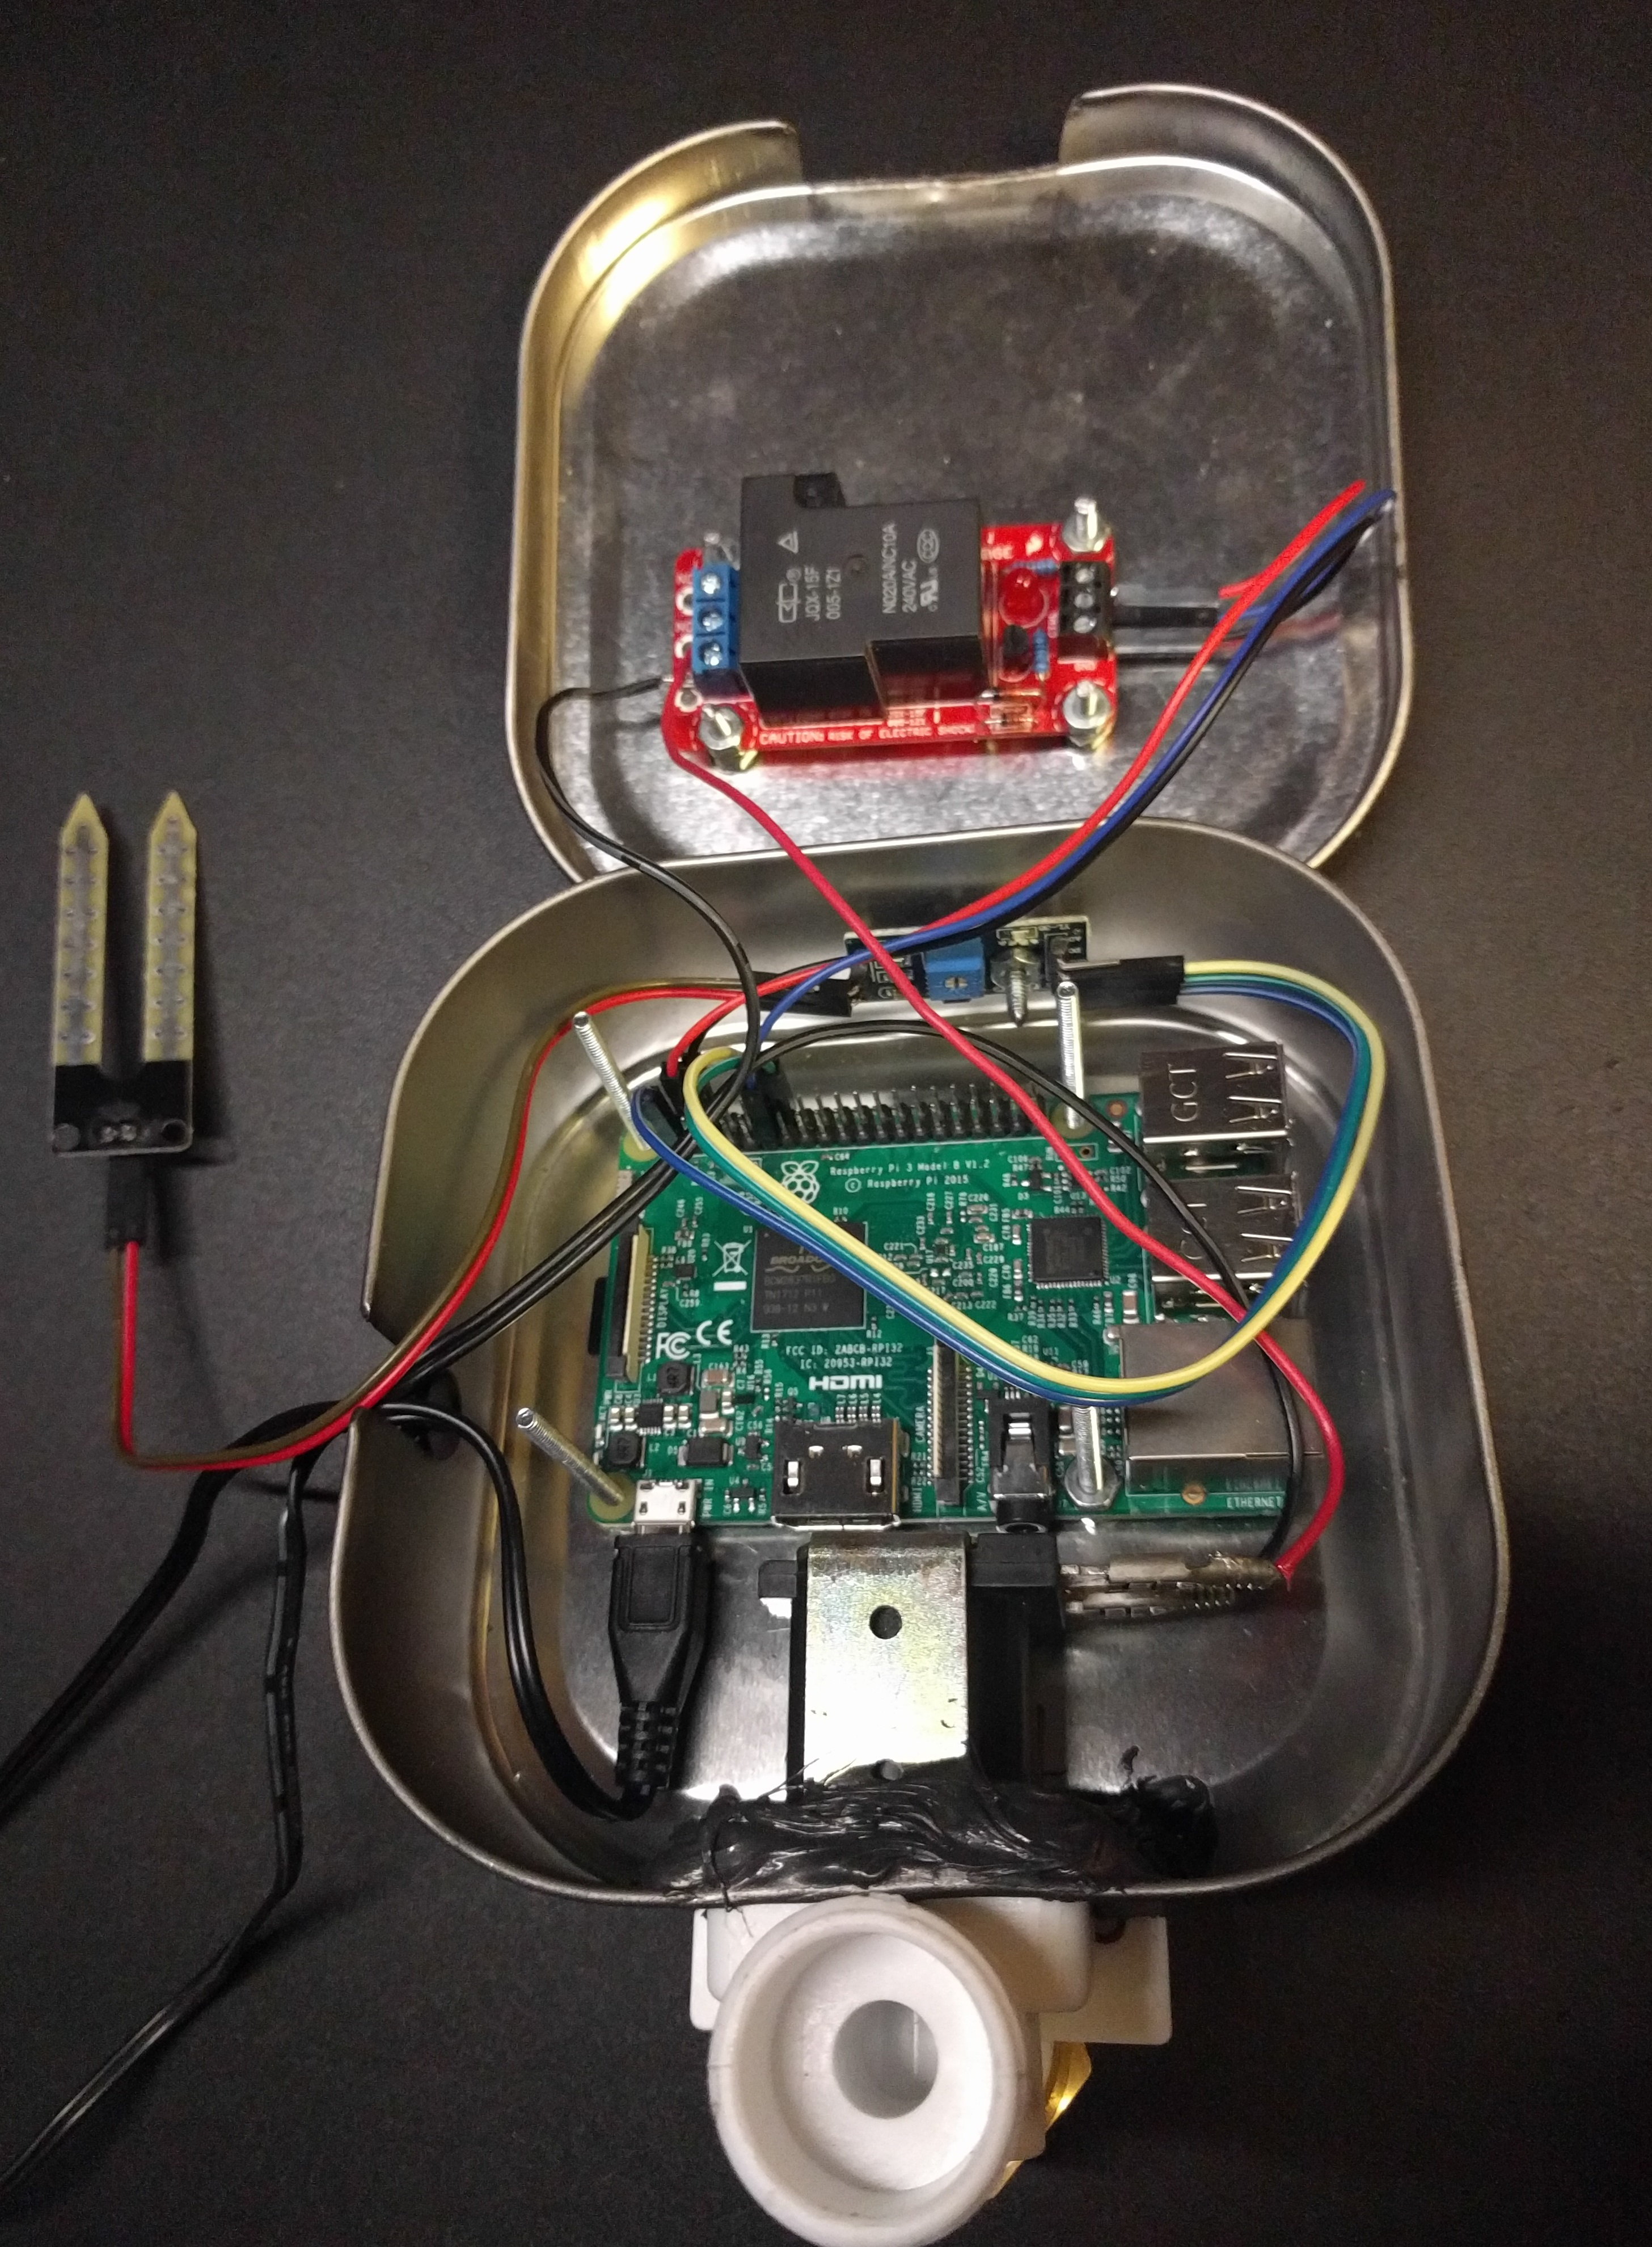
\includegraphics[height=7cm]{../img/the-guts}
        \caption{The insides of the "black box"}
    \end{figure}
\end{frame}

\begin{frame}
    \frametitle{Hardware Construction} % in place
    \begin{figure}
        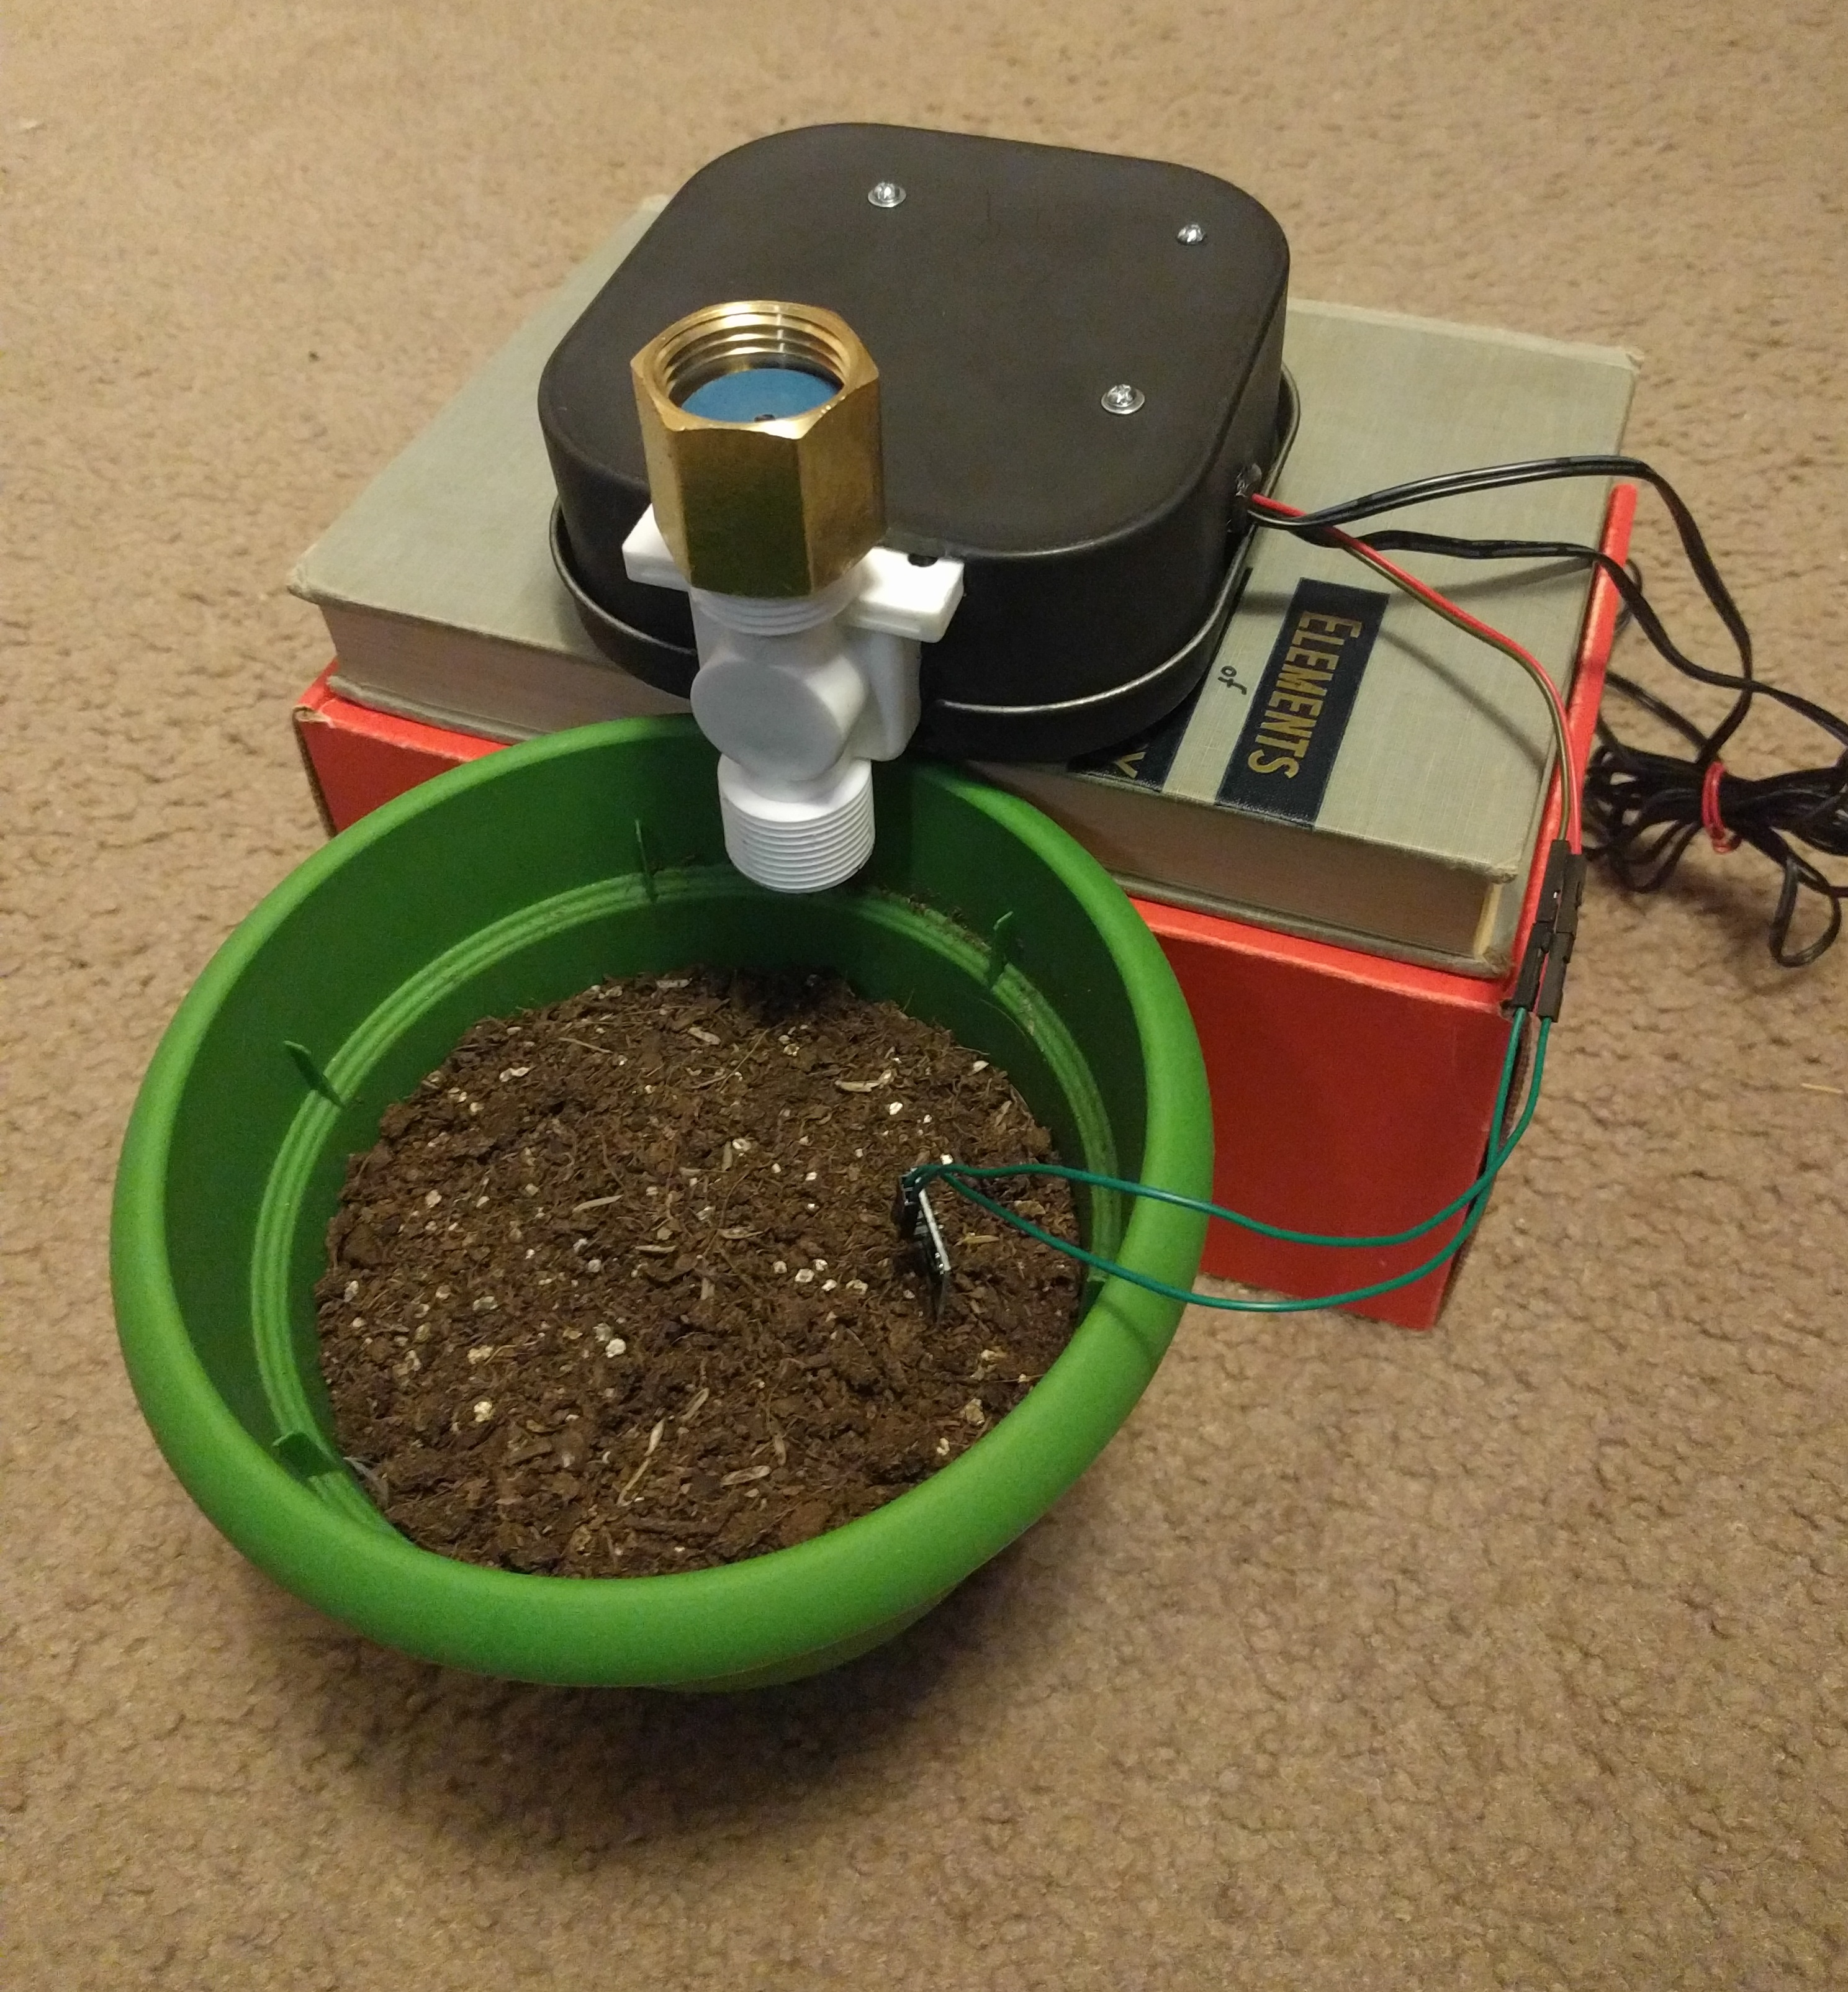
\includegraphics[height=7cm]{../img/in-use}
        \caption{The watering system in place}
    \end{figure}
\end{frame}

\begin{frame}
    \frametitle{Wiring Diagram}
    \begin{figure}
        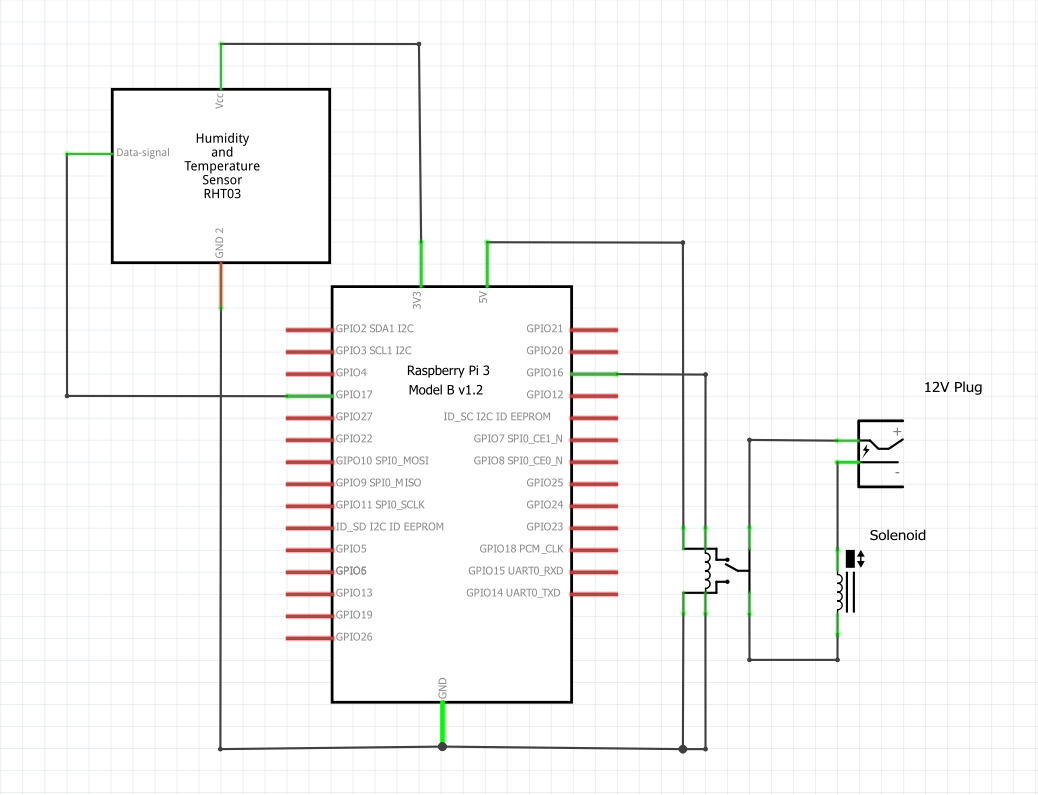
\includegraphics[height=7cm]{../img/circuit}
        \caption{The system's circuit diagram}
    \end{figure}
\end{frame}

\begin{frame}
    \frametitle{Software}
    \begin{minipage}{0.52\textwidth}
        \begin{itemize}
            \item Still a work in progress
            \item Once per hour, the RasPi polls the data pin on the hygrometer
            \item If the reading is below a pre-defined threshold, the RasPi opens the
                  solenoid for 5 seconds
            \item (Repeat, ad infinitum)
        \end{itemize}
    \end{minipage}%
    \begin{minipage}{0.45\textwidth}
        
\includegraphics[width=5.5cm]{../img/matrix}
    \end{minipage}%
\end{frame}

\begin{frame}
    \frametitle{Challenges}
    \begin{itemize}
        \item I wasn't able to find a 5V solenoid to run straight off of the Pi board
        \item This necessitated adding a relay, which was more of an annoyance than a huge hurdle
        \pause
        \item The solenoid I did get requires high water pressure to operate, so it needs to connect
              to a faucet, rather than be gravity fed
        \pause
        \item Basically, the solenoid was a pain
    \end{itemize}
\end{frame}

\begin{frame}
    \frametitle{Live Demo?}
    \begin{itemize}
        \item Sadly, not today...
        \pause
        \item The solenoid requires relatively high water pressure, which can't
            be easily achieved in the classroom
        \item I also have a bad solder joint that needs fixing first
    \end{itemize}
\end{frame}

\begin{frame}
    \frametitle{Questions?}
    \begin{figure}
        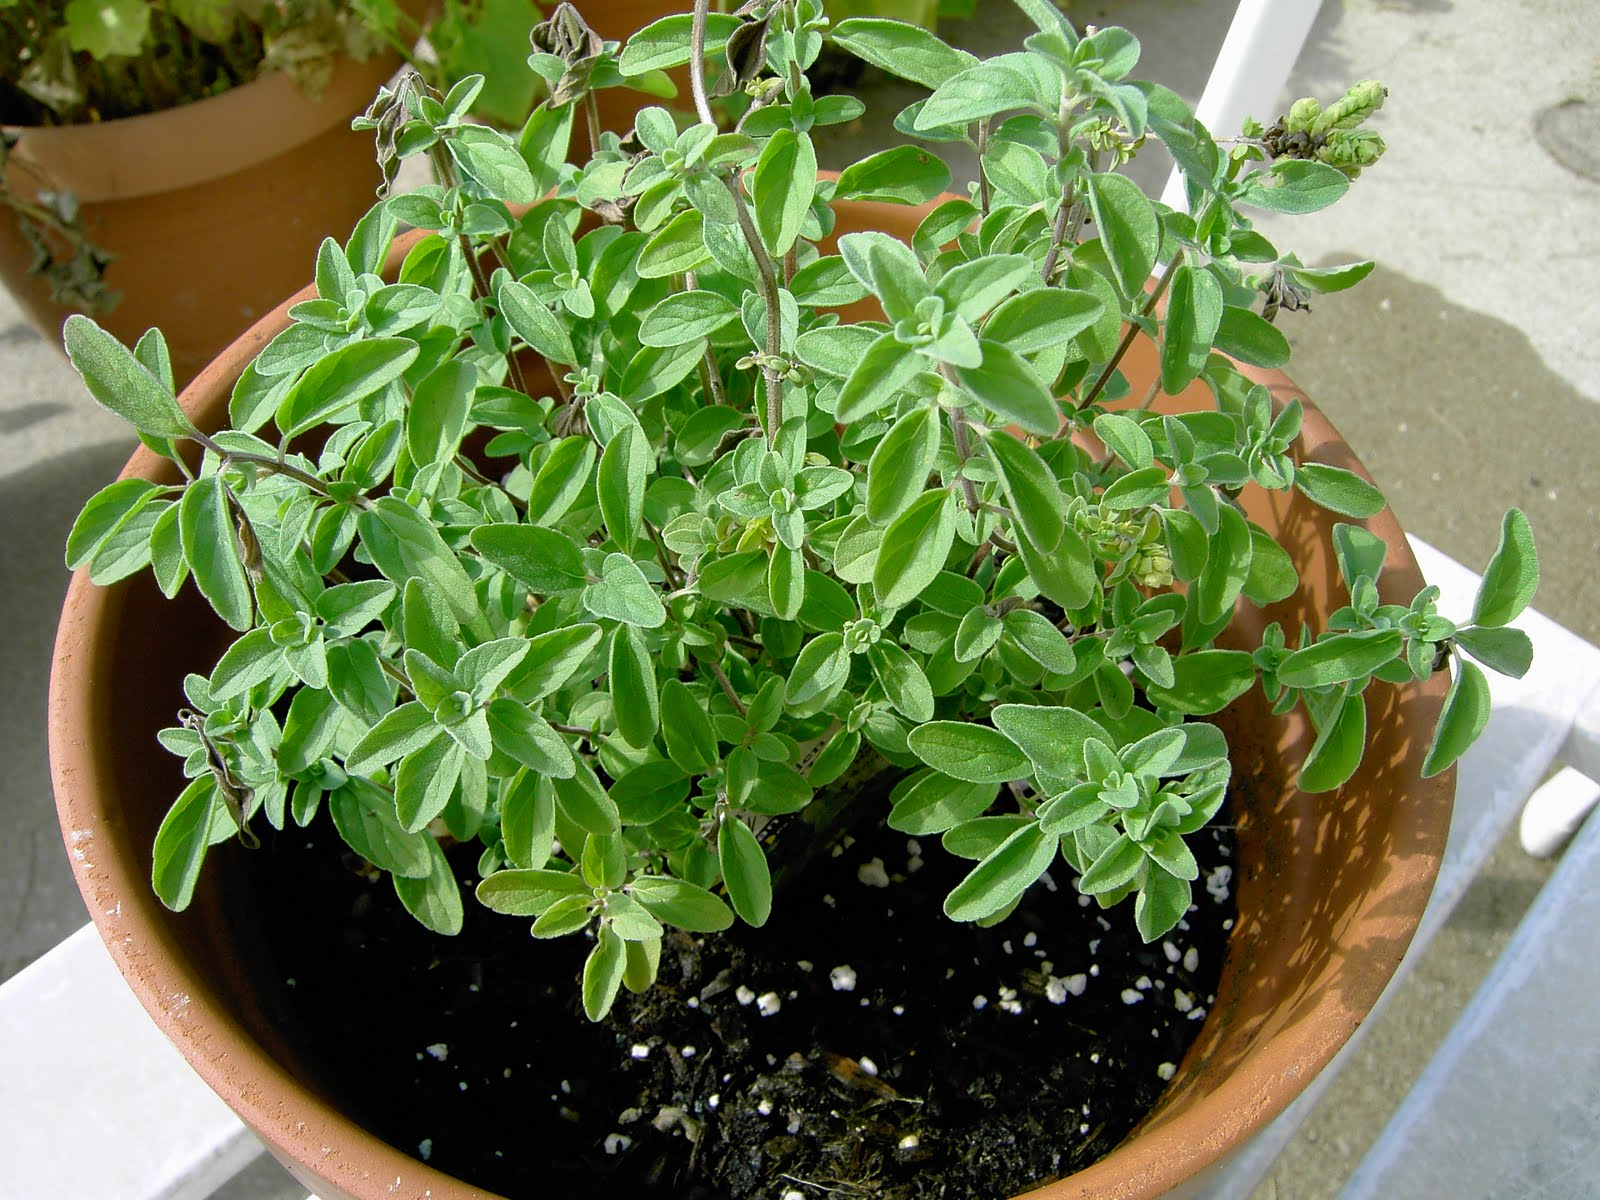
\includegraphics[width=9cm]{../img/happy-plants}
        \caption{Healthy plants!}
    \end{figure}
\end{frame}


\end{document}
